\chapter[Grundlagen]{Grundlagen}

Ziel dieses Kapitels ist die Erläuterung von notwendigen Konzepten zur weiteren Betrachtung des Themas Integration der Data Science in Organisationen und Abteilungen.
Dazu werden in diesem Kapitel besonders auf die zwei grundlegenden Thematiken der Data Science und der allgemeinen Betrachtung von Organisationen eingegangen.

\section{Disziplin der Data Science}

Dieser Abschnitt des Kapitels beleuchtet zunächst die Disziplin der Data Science.
Wie in der Problemstellung identifiziert steigt das Interesse an der Aufzeichnung und Verarbeitung von Daten innerhalb von Organisationen. 
Da hierfür folglich qualifiziertes Fachpersonal benötigt wird nimmt auch die Rolle des Data Scientist an Wert für Unternehmen zu. \footcite[prenote][postnote]{the role of data scientists}
Aufgabe dieser Rolle ist es an Datenanwendungen zu arbeiten, welche eine zeitnahe signifikante Auswirkung auf das Geschäftsmodell verursachen. \footcite[prenote][postnote]{aim of data scientists}
Data Science im Allgemeinen wird häufig mit einem Prozess in Verbindung gebracht, welcher durch Einsatz von Techniken des maschinellen Lernens wichtige Erkenntnisse aus Daten ableitet. \footcite[prenote][postnote]{data science often refers}
van der Aalst definierte im Jahr 2016 das Feld der Data Science wie folgt: \cite[prenote][postnote]{data science definition}

\begin{quotation}
    \textit{
    Data science is an interdisciplinary field aiming to turn data into real value.
    Data may be structured or unstructured, big or small, static or streaming.
    Value may be provided in the form of predictions, automated decisions, models learned from data, or any type of data visualization delivering insights.
    Data science includes data extraction, data preparation, data exploration, data transformation, storage and retrieval, computing infrastructures, various types of mining and learning, presentation of explanations and predictions, and the exploitation of results taking into account ethical, social, legal, and business aspects.    
    }
\end{quotation}

Die Definition betrachtet die drei wichtigen Aspekte der Daten, des Wertbeitrags und der Aufgabenbereiche.
Folgend werden die einzelnen Aspekte, ausgeschlossen des bereits im vorherigen Kapitel behandelten Wertbeitrags, detaillierter ausgeführt.

% Daten
Aus der Definition lassen sich bereits einige Charakteristika von Daten hinsichtlich Form, Menge und Persistenz erkennen.
In der Literatur werden besonders im Bereich von \textit{Big Data} die 5 V's von Daten thematisiert.
Übersetzt beschreiben sie die Charakteristika Volumen, Geschwindigkeit, Wahrheit, Vielfalt und Wert. \footcite[prenote][postnote]{Big data is always}
Ausprägungen dieser Merkmale lassen sich wie folgt zuordnen: Volumen - Number of Bytes, Geschwindigkeit - static or real time, Richtigkeit - Grad der Vorurteilsbehaftung, Vielfalt - strukturiert oder unstrukturiert, Wert - Leistungspotenzial der Daten.
Von diesen Charakteristika liegt jedoch global betrachtet der Großteil der Daten in unstrukturierter Form, bspw. als Text, Bild oder Audio, vor. \footcite[prenote][postnote]{most of the data}

% Disziplin / Aufgabenbereich
Die Disziplin der Data Science entwickelte sich aus der Statistik und der Kombination vieler verwandter Disziplinen, welche selbst unter sich Überschneidungen aufweisen und in ihrem Einfluss auf die Data Science variieren. \footcite[prenote][postnote]{disciplines of data science}
Die verwandten Wissenschaftsbereiche sind dabei in Abbildung \textbf{X} aufgezeigt. \footcite[prenote][postnote]{disciplines of data science}

\begin{figure}[htb]
    \centering
    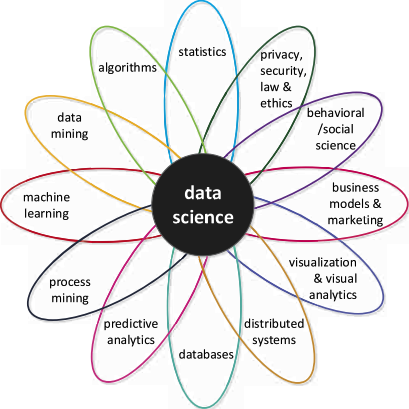
\includegraphics[width=0.5\textwidth]{graphics/ds_disciplines.png}
    \caption{Disziplinen der Data Science}
    \label{fig:data science disciplines}
\end{figure}

Anwendung der Data Science und deren Subdisziplinen findet sich in der Bearbeitung von datengetriebenen Problemstellungen der vier Kategorien: Berichterstattungen, Diagnosen, Vorhersagen und Empfehlungen. \footcite[prenote][postnote]{four main categories}
Als Arbeitsablauf dieser Bearbeitung wird in der Literatur häufig ein Prozess mit drei Phasen und bis zu zehn Schritten beschrieben, welcher die Phasen der Datenvorbereitung, der Modellentwicklung und dessen Bereitstellung involviert. \footcite[prenote][postnote]{data science process as roughly 3}
Dabei ist es sinnvoll je nach Anwendung und Problemstellung verschiedene Phasen zu fokussieren.
Beispielsweise sind zur Berichterstattung die Datenvorbereitung und Bereitstellung der Erkenntnisse zu fokussieren, da häufig kein explizites Modell zu entwickeln ist.
Hingegen werden bei der Erstellung von Vorhersagen und Empfehlungen akkurate Modelle benötigt, um die Richtigkeit der Vorhersagen und Empfehlungen zu garantieren.
Konkrete Aufgaben in der Data Science Rolle umfassen das Bereinigen und Vereinen von Datensätzen, die Visualisierung von Daten oder die Entwicklung umfangreicher Softwaretools zur Verarbeitung von Daten. \footcite[prenote][postnote]{tasks of a data scientist}

\section{Organisationen}

\section{Abgrenzung von datengesteuerten Organisationen}